\documentclass[12pt]{article}
\usepackage{polski}
\usepackage[utf8]{inputenc}
\usepackage{amsfonts}
\usepackage{amsmath}
\usepackage{enumitem}
\usepackage{graphicx}
\setlength{\parskip}{1em}


\begin{document}
	\title{Sprawozdanie\\Metody Numeryczne 2, laboratorium 1}
	\author{Grzegorz Rozdzialik (D4, grupa lab. 2)}
	\maketitle	
	
	\section{Zadanie}
	{\Large Temat \textbf{2}, zadanie \textbf{49}:}\\
	Interpolacja funkcjami liniowymi na kwadracie podzielonym na $2n^2$ trójkątów przystających. Zagęszczanie podziału kwadratu, aż do osiągnięcia błędu średniokwadratowego, mierzonego w środkach ciężkości trójkątów, mniejszego od $\varepsilon$.
	
	\section{Opis metody}
	Mając funkcję interpolowaną $f: D \to \mathbb{R}$, gdzie $D = \{ (x, y) \in \mathbb{R}^2: x_0 \leq x \leq x_0 + H, y_0 \leq y \leq y_0 + H\}$, $H, x_0, y_0 \in \mathbb{R}$ opisaną na kwadracie o boku $H$, którego lewy dolny wierzchołek ma współrzędne $(x_0, y_0)$, należy skonstruować funkcję sklejaną $p: D \to \mathbb{R}$ złożoną z funkcji opisanych na pojedynczych trójkątach przystających, dzielących ten kwadrat.
	
	\begin{figure}[]
		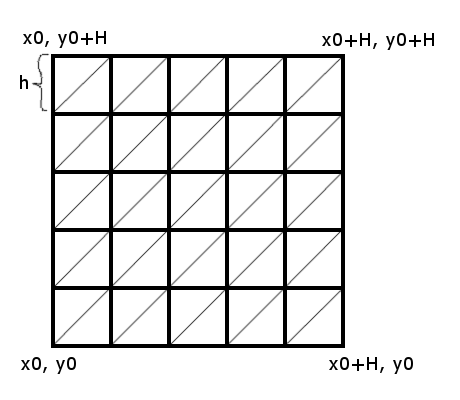
\includegraphics[scale=0.8]{square-division.png}
		\caption{Przedstawienie podziału dziedziny funkcji $f$}
	\end{figure}
	
	Dziedzinę funkcji $f$ należy podzielić na $n$ części wzdłuż osi $x$ oraz osi $y$, co daje $n^2$ kwadratów, a następnie każdy kwadrat można podzielić względem dowolnej przekątnej na dwa trójkąty. W moim rozwiązaniu użyłem przekątnej o współczynniku kierunkowym równym $1$.
	
	\section{Implementacja metody}
	Przyjmijmy, że punkt $(x_0, y_0) \in D$ to lewy dolny wierzchołek dziedziny. Startując z parametrem $n = 1$ należy podzielić kwadrat na $n^2$ kwadratów przystających ($n$ podziałów wzdłuż osi X, $n$ podziałów wzdłuż osi Y), a następnie podzielić każdy z nich na dwa prostokątne trójkąty przystające, których przeciwprostokątną będzie przekątna kwadratu o współczynniku kierunkowym równym $1$.
	
	Niech $h = \frac{H}{n}$ będzie długością boku każdego z mniejszych kwadratów.
	
	Rozważmy jeden z kwadratów po podziale, będący w $i$-tym rzędzie i $j$-tej kolumnie. Wtedy jego lewy dolny wierzchołek ma współrzędne $(a, b) = (x_0 + j*h, y_0 + i*h)$.
	
	Wierzchołki trójkąta powyżej przekątnej kwadratu mają współrzędne $(a, b)$, $(a + h, b + h)$, $(a, b + h)$, a jego środek ciężkości znajduje się w punkcie $(a + \frac{h}{3}, b + \frac{2}{3}h)$.
	
	Wierzchołki trójkąta poniżej przekątnej kwadratu mają współrzędne $(a, b)$, $(a + h, b)$, $(a + h, b + h)$, a jego środek ciężkości znajduje się w punkcie $(a + \frac{2}{3}*h, b + \frac{h}{3})$.
	
	Na rysunku 2 rozstał przedstawiony podział kwadratu na dwa trójkąty przystające, oraz środek ciężkości jednego z trójkątów.
	
	\pagebreak
	
	\begin{figure}
		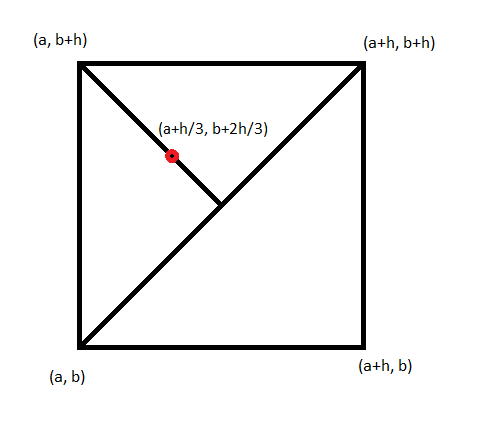
\includegraphics[scale=1]{images/single-square-gravity-center.png}
		\caption{Środek ciężkości trójkąta dzielącego kwadrat}
	\end{figure}
	
	Interpolacja będzie za pomocą funkcji liniowych, więc każda z funkcji $p$ ma równanie:
	$$p(x, y) = \alpha_0 + \alpha_1*x + \alpha_2*y$$
	gdzie $\alpha_0, \alpha_1, \alpha_2$ są współczynnikami specyficznymi dla danego trójkąta, na którym się odbywa interpolacja.
	
	Biorąc wierzchołki trójkątów za węzły interpolacji i korzystając z założenia, że dla węzłów interpolacji spełniony jest warunek:
	$$p(x_i, y_i) = f(x_i, y_i)$$
	gdzie $(x_i, y_i)$ jest węzłem interpolacji, otrzymujemy następujący układ równań:
	\begin{align*}
		\left[
			\begin{array}{ccc}
				1 &  a  &  b  \\
				1 & a+h &  b  \\
				1 & a+h & b+h
			\end{array}
		\right]
		\left[
			\begin{array}{c}
				\alpha_0 \\
				\alpha_1 \\
				\alpha_2
			\end{array}
		\right]
		=		
		\left[
			\begin{array}{c}
				  f(a, b)   \\
				 f(a+h, b)  \\
				f(a+h, b+h)
			\end{array}
		\right]
	\end{align*}
	dla trójkąta powyżej przekątnej, oraz:
	\begin{align*}
		\left[
			\begin{array}{ccc}
				1 &  a  &  b  \\
				1 & a+h &  b  \\
				1 & a+h & b+h
			\end{array}
		\right]
		\left[
			\begin{array}{c}
				\alpha_0 \\
				\alpha_1 \\
				\alpha_2
			\end{array}
		\right]
		=		
		\left[
			\begin{array}{c}
				  f(a, b)   \\
				 f(a+h, b)  \\
				f(a+h, b+h)
			\end{array}
		\right]
	\end{align*}
	dla trójkąta poniżej przekątnej. Rozwiązując te układy równań otrzymujemy współczynniki potrzebne do wyznaczenia funkcji interpolującej $p$.
	
	\section{Warunek stopu}
	Podział zagęszczamy (zwiększamy parametr $n$), dopóki błąd średniokwadratowy mierzony w środkach ciężkości trójkątów jest większy od zadanej dokładności $\varepsilon$.
	
	Obliczenia kontynuujemy dopóki spełniony jest warunek:
	\begin{align*}
		\frac{\sum_{(x_j, y_i)} (f(x_j, y_i) - p(x_j, y_i))^2}{2n^2} \geq \varepsilon
	\end{align*}
	gdzie punkty $(x_j, y_i)$ są środkami ciężkości kolejnych trójkątów.
	
	\section{Poprawność metody}
	Metoda na ogół jest poprawna, jednak podczas testów zdarzało się tak, że funkcja interpolująca $p$ nie miała odległych wartości w środkach ciężkości trójkątów, a poza nimi znacznie różniła się od funkcji interpolowanej $f$. Oznaczało to, że warunek stopu został osiągnięty po zaledwie kilku próbach ($n$ około 3), natomiast interpolacja była niedokładna.
	
	Były to jednak nieliczne przypadki. W większości metoda zachowywała się poprawnie i dawała dobre wyniki.
	
	\section{Przykłady}
	\begin{enumerate}[label=\textbf{Przykład \arabic*}]
		\item
		Funkcja $f(x, y) = x^2 + y^2$.\\
		Lewy dolny wierzchołek kwadratu: $(0, 0)$.\\
		Długość boku kwadratu: $2$.\\
		$\varepsilon = 0.1$
		
		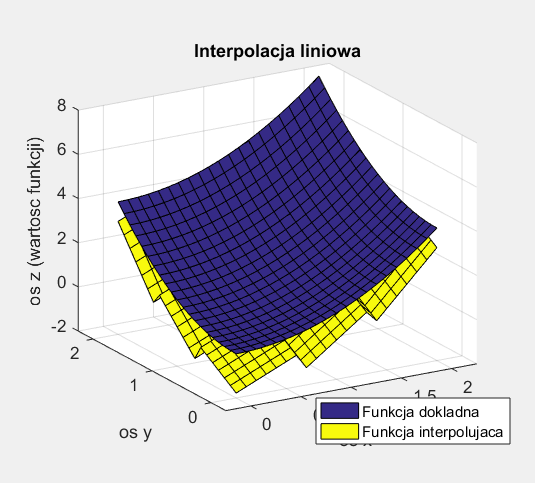
\includegraphics[]{images/example-1.png}
		
		\textbf{Wyniki}:\\
		Osiągnięto zadaną dokładność przy $n = 3$ ($18$ trójkątów przystających).\\
		Podział trwał $1.006080$ ms.\\
		Obliczanie ostatecznych współczynników dla funkcji interpolujących trwało $0.316587$ ms.\\
		Sprawdzanie ostatecznego błędu interpolacji trwało $0.025173$ ms.\\
		Osiągnięto błąd interpolacji równy $0.0390184$ (zadano $0.1$).\\
		Obliczanie wartości do wykresu trwało $0.468480$ ms.
		
		
		
		\item
		Funkcja $f(x, y) = x^2 + y^2$.\\
		Lewy dolny wierzchołek kwadratu: $(0, 0)$.\\
		Długość boku kwadratu: $2$.\\
		$\varepsilon = 0.01$
		
		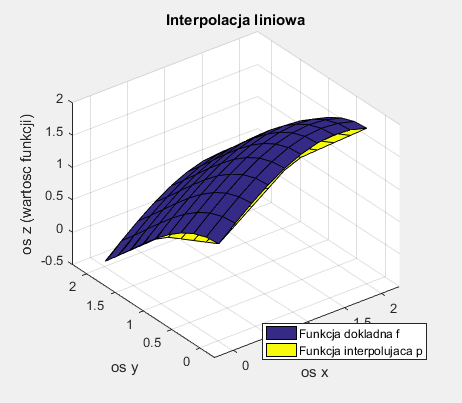
\includegraphics[]{images/example-2.png}
		
		\textbf{Wyniki}:\\
		Osiągnięto zadaną dokładność przy $n = 5$ ($50$ trójkątów przystających).\\
		Podział trwał $5.291949$ ms.\\
		Obliczanie ostatecznych współczynników dla funkcji interpolujących trwało $1.093547$ ms.\\
		Sprawdzanie ostatecznego błędu interpolacji trwało $0.121600$ ms.\\
		Osiągnięto błąd interpolacji równy $0.00505679$ (zadano $0.01$).\\
		Obliczanie wartości do wykresu trwało $0.713387$ ms.
		
		
		
		\item
		Funkcja $f(x, y) = x^2 + y^2$.\\
		Lewy dolny wierzchołek kwadratu: $(0, 0)$.\\
		Długość boku kwadratu: $2$.\\
		$\varepsilon = 10^{-5}$
		
		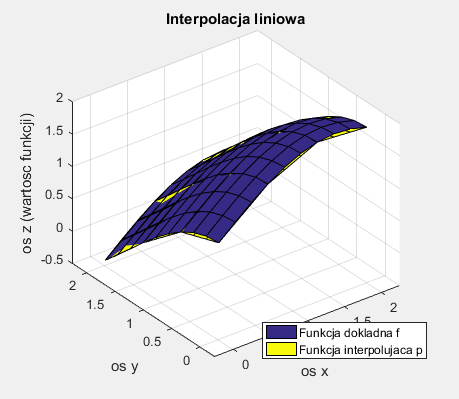
\includegraphics[]{images/example-3.png}
		
		\textbf{Wyniki}:\\
		Osiągnięto zadaną dokładność przy $n = 24$ ($1152$ trójkątów przystających).\\
		Podział trwał $187.255973$ ms.\\
		Obliczanie ostatecznych współczynników dla funkcji interpolujących trwało $23.461557$ ms.\\
		Sprawdzanie ostatecznego błędu interpolacji trwało $1.129387$ ms.\\
		Osiągnięto błąd interpolacji równy $9.52599e-06$ (zadano $1e-05$).\\
		Obliczanie wartości do wykresu trwało $0.538027$ ms.
		
		
		
		\item
		Funkcja $f(x, y) = x^2 + y^2$.\\
		Lewy dolny wierzchołek kwadratu: $(0, 0)$.\\
		Długość boku kwadratu: $10$.\\
		$\varepsilon = 10^{-5}$
		
		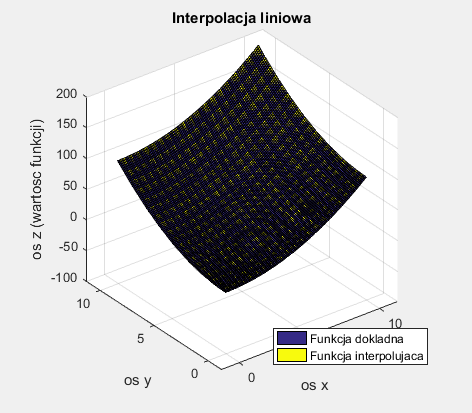
\includegraphics[]{images/example-4.png}
		
		\textbf{Wyniki}:\\
		Osiągnięto zadaną dokładność przy $n = 119$ ($28322$ trójkątów przystających).\\
		Podział trwał $17248.057768$ ms.\\
		Obliczanie ostatecznych współczynników dla funkcji interpolujących trwało $403.329582$ ms.
		Sprawdzanie ostatecznego błędu interpolacji trwało $29.678268$ ms.\\
		Osiągnięto błąd interpolacji równy $9.85025 * 10^{-6}$ (zadano $10^{-5}$).\\
		Obliczanie wartości do wykresu trwało $8.104837$ ms.
		
		
		
		\item
		Funkcja: $f(x, y) = \sin x + \cos y$.\\
		Lewy dolny wierzchołek kwadratu: $(0, 0)$.\\
		Długość boku kwadratu: $10$.\\
		$\varepsilon = 0.1$
		
		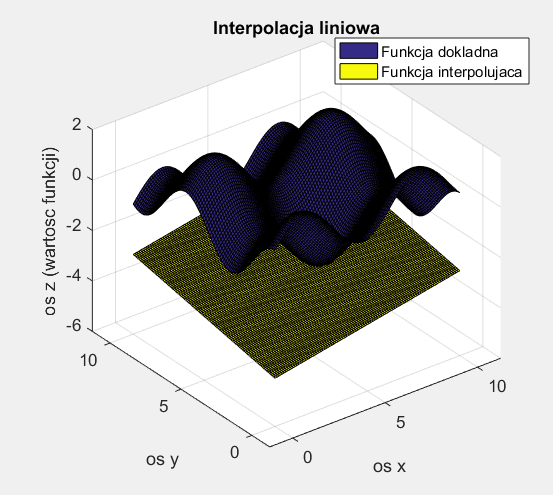
\includegraphics[]{images/example-5.png}
		
		\textbf{Wyniki}:\\
		Osiągnięto zadaną dokładność przy $n = 1$ ($2$ trójkąty przystające).\\
		Podział trwał $0.212907$ ms.\\
		Obliczanie ostatecznych współczynników dla funkcji interpolujących trwało $0.145067$ ms.\\
		Sprawdzanie ostatecznego błędu interpolacji trwało $0.023893$ ms.\\
		Osiągnięto błąd interpolacji równy $0.0224202$ (zadano $0.1$).\\
		Obliczanie wartości do wykresu trwało $9.846618$ ms.
		
		
		\item
		Funkcja: $f(x, y) = \sin x + \cos y$.\\
		Lewy dolny wierzchołek kwadratu: $(0, 0)$.\\
		Długość boku kwadratu: $10$.\\
		$\varepsilon = 0.01$
		
		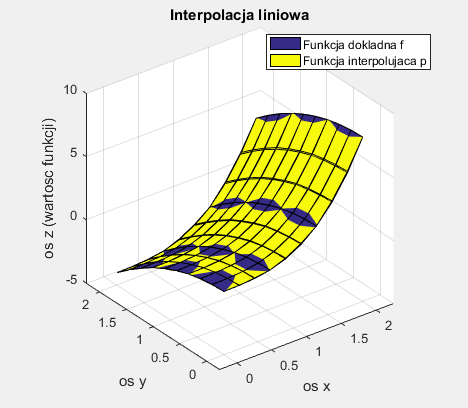
\includegraphics[]{images/example-6.png}
		
		\textbf{Wyniki}:\\
		Osiągnięto zadaną dokładność przy $n = 11$ ($242$ trójkątów przystających).\\
		Podział trwał $22.700810$ ms.\\
		Obliczanie ostatecznych współczynników dla funkcji interpolujących trwało $4.952749$ ms.\\
		Sprawdzanie ostatecznego błędu interpolacji trwało $0.351147$ ms.\\
		Osiągnięto błąd interpolacji równy $0.00791773$ (zadano $0.01$).\\
		Obliczanie wartości do wykresu trwało $11.321605$ ms.
		
		
	\end{enumerate}
	
	\section{Wnioski}
	\begin{enumerate}
		\item Wraz ze zmniejszaniem parametru $\varepsilon$ wykres funkcji interpolującej $p$ zbliża się do wykresu funkcji interpolowanej $f$ (przykłady 1, 2 oraz 3).
		
		Wraz ze zwiększaniem się dokładności, czas potrzebny na otrzymanie zadanej dokładności wygląda, jakby wzrastał wykładniczo.
		
		Zależności z tych przykładów te zostały pokazane na wykresach znajdujących się na rysunkach 3 oraz 4.
		
		
		\begin{figure}
			\centering
			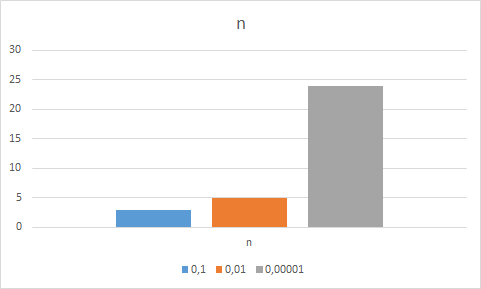
\includegraphics[]{images/wykres-n.png}
			\caption{Wykres liczby $n$ w zależności od zadanej dokładności $\varepsilon$}
			
			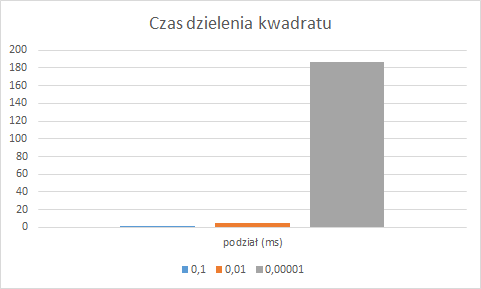
\includegraphics[]{images/wykres-czas-dzielenia.png}
			\caption{Wykres czasu podziału kwadratu w zależności od zadanej dokładności $\varepsilon$}
		\end{figure}

		\item Osiągnięcie dużej dokładności (poniżej $\varepsilon = 10^{-4}$) na dużym obszarze ($H \geq 10$) wymaga sporej ilości obliczeń (przykład 4).
		
		\item Istnieją funkcje, które szybko osiągają warunek stopu, ponieważ funkcja interpolująca osiąga wartości zbliżone do dokładnych w środkach ciężkości, natomiast znacznie inne poza nimi. Prezentujące to przykłady mają numery 5 oraz 6. W przykładzie 5-tym funkcja interpolująca $p$ w ogóle nie przypomina funkcji interpolowanej $f$, ponieważ kwadrat, na którym odbywała się interpolacja został podzielony jedynie na dwa trójkąty, dla których warunek stopu został od razu spełniony. Funkcja interpolująca z przykładu 6 dużo lepiej odwzorowuje funkcję interpolowaną.
	\end{enumerate}

	\pagebreak
	
	\section{Funkcja do testowania}
	Do sprawdzenia funkcji, które nie zostały udostępnione w interfejsie graficznym należy wykorzystać funkcję $interpolateSquare(f, x0, y0, H, n, epsilon, log, displayType)$. Ta funkcja udostępnia funkcjonalność analogiczną do interfejsu graficznego.
	
	Więcej informacji dotyczących wykorzystania funkcji $interpolateSquare$ znajduje się w pliku z funkcją (\textit{interpolateSquare.m}).
	
	\section{Interfejs graficzny}
	Do metody został dodany interfejs graficzny, umożliwiający wygodne testowanie metody dla różnych parametrów i różnych funkcji interpolowanych $f$. Aby go wywołać należy uruchomić komendę \textit{interpolationGUI} w MATLABie.
	
	\begin{figure}
		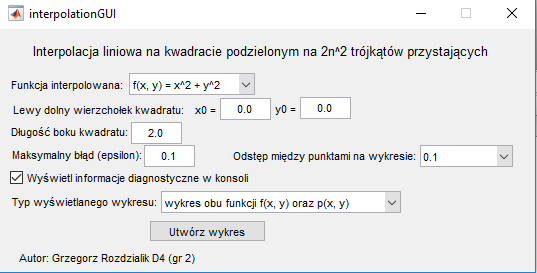
\includegraphics[scale=1]{images/gui.png}
		\caption{Interfejs graficzny}
	\end{figure}
	
	\section{Bibliografia}
	\begin{enumerate}
		\item Książka (dopisać)
		\item Informacje z wykładu
		\item Dopisać wikipedię albo coś takiego
	\end{enumerate}
	
\end{document}